% Chapter 5

\chapter{Produzione} % Main chapter title

\label{Chapter5} % Change X to a consecutive number; for referencing this chapter elsewhere, use \ref{ChapterX}

%----------------------------------------------------------------------------------------
%	SECTION 1
%----------------------------------------------------------------------------------------

\section{Modellazione}
\begin{itemize}
    \item modelli "lowpoly"
\end{itemize}
\section{Texturing}
\section{Animazione e Rigging}

\begin{figure}
\centering
\begin{subfigure}{.33\textwidth}
  \centering
  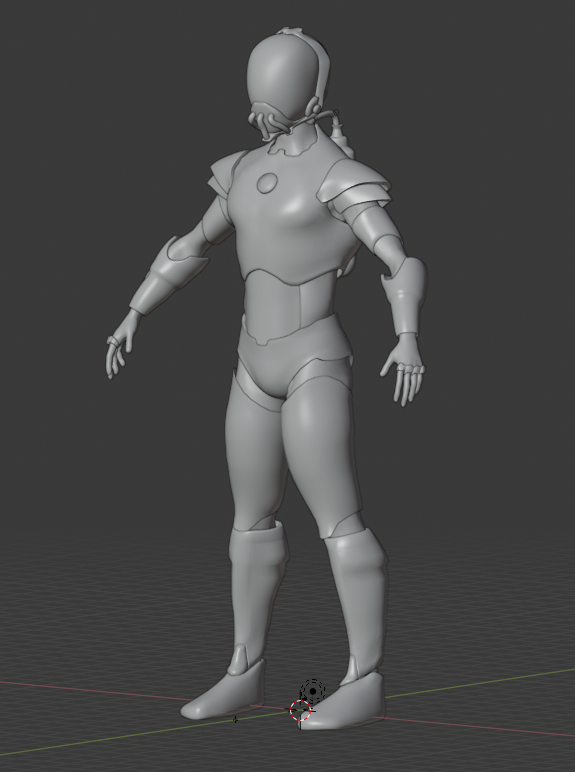
\includegraphics[width=\linewidth]{Figures/rig0}
  \caption{Modello senza controlli.\\}
  \vspace{13pt}
  \label{fig:rig0}
\end{subfigure}%
\begin{subfigure}{.33\textwidth}
  \centering
  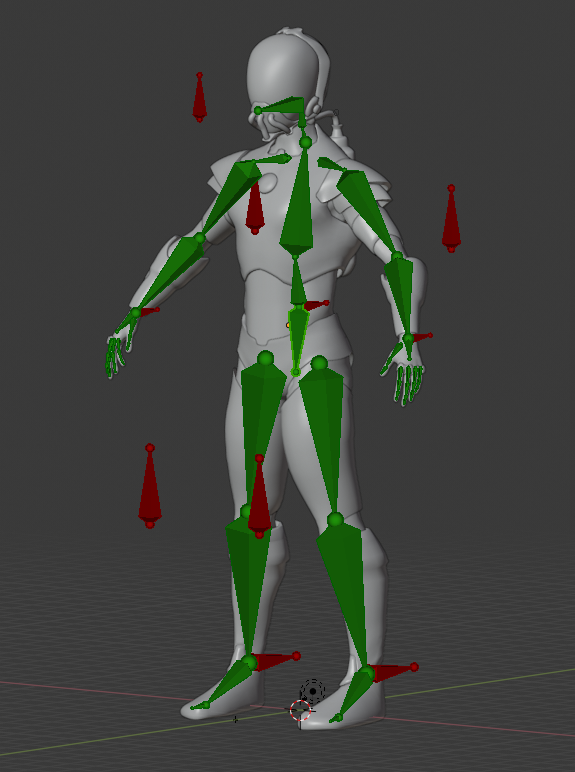
\includegraphics[width=\linewidth]{Figures/rig1}
  \caption{Armatura o meta-rig.}
  \bigskip
  \label{fig:rig1}
\end{subfigure}%
\begin{subfigure}{.33\textwidth}
  \centering
  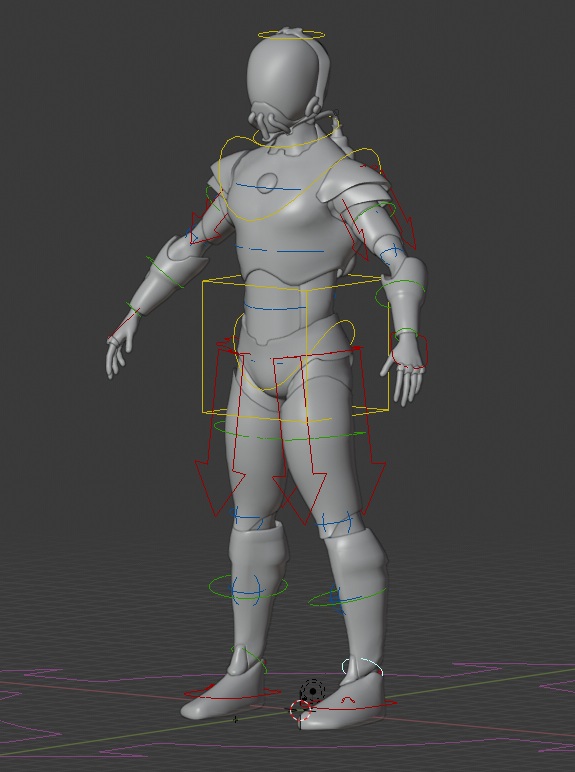
\includegraphics[width=\linewidth]{Figures/rig2}
  \caption{Rig avanzato con forme personalizzate.}
  \label{fig:rig2}
\end{subfigure}
\decoRule
\caption[Confronto di rig]{In figura è mostrato il modello di uno dei personaggi, con diversi tipi di controlli per l'animazione.}
\label{fig:rig}
\end{figure}

Rigging è un termine generale che si riferisce all'aggiunta di controlli ad un oggetto, tipicamente allo scopo di animarlo \parencite{blendDoc}.
Consiste nell'assegnare relazioni tra oggetti \parencite{BlendTut}.

Animazione straight ahead vs pose-to-pose (mixing between the 2)

uso di shape keys
ogni vertice è importante, inutile associare un'osso per ogni gruppo di vertici: meglio avere diverse espressioni (set finito) e sciegliere quale si vuole usare in ase ad un valore reale (continuo)

dialoghi
menzionare Rhubarb

divisione dx/sx

\subsection{Cicli di animazione}
Il miglior modo per modulare un animazione, ovvero spezzarla in più azioni ripetibili, è quello di individuare le animazioni più frequenti (e.g. camminata, corsa) e definirle una sola volta.
Alcune animazioni, infatti, seguono dei pattern ben definiti.
Grazie alla loro uniformità è possibile renderle cicliche in maniera tale da non dover rifare la stessa animazione più volte.
\subsection{Shape keys}
Facial expression
uso di shape keys
ogni vertice è importante, inutile associare un osso per ogni gruppo di vertici: meglio avere diverse espressioni (set finito) e scegliere quale si vuole usare in base ad un valore reale (continuo)
\subsection{Drivers}
\subsection{Vincoli sulle azioni}
uno dei vantaggi dei vincoli sulle azioni è che è possibile animare le ossa vincolate direttamente, senza aggiungere un osso padre.

Solitamente utilizzate per controllare animazioni molto complesse, come la fuoriuscita del carrello di un aereo al momento dell'atterraggio, attraverso un solo controllo.

Reference
\begin{itemize}
    \item Dialog - The Animator's Survival Kit (p.304) 
    \item Facial animation - Algorithms\&Techniques (p.491)
    \item cycles - Finish you film (Production)
\end{itemize}
\section{Lighting}
\section{Rendering}

